\subsection{Arquitectura de conversión de datos}

La arquitectura del Modelo de Información de Integración de openEHR, mostrada en la Figura \ref{fig:data_conversion_architecture}, está diseñada para situaciones de integración heredadas.

\begin{figure}[h]
  \centering
  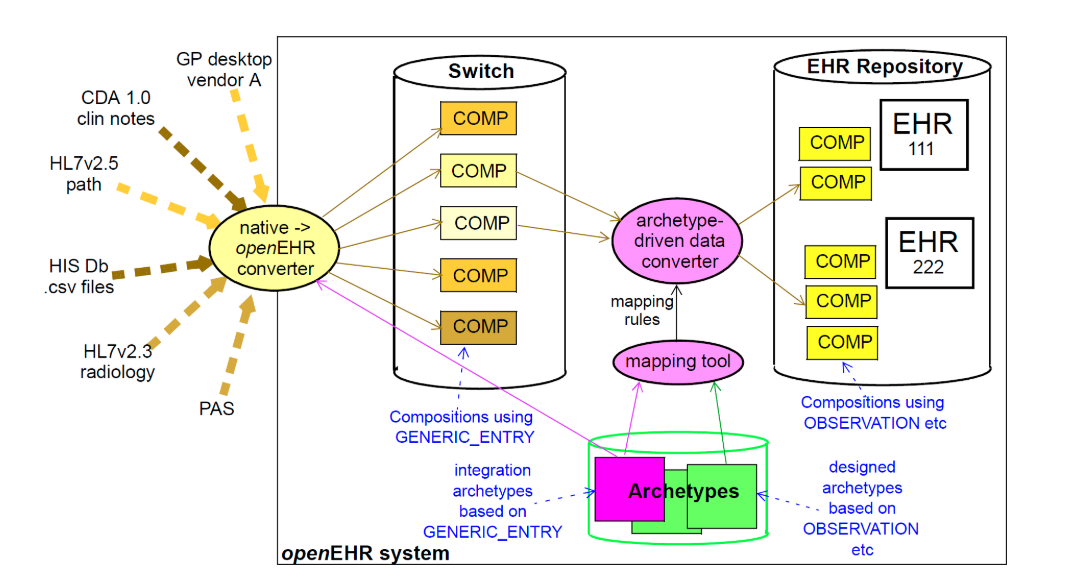
\includegraphics[scale=0.4]{./images/data_conversion_architecture}
  \caption{Integración de dato dentro de openEHR (Fuente: Extraído desde \cite{openEHR}).}
  \label{fig:data_conversion_architecture}
\end{figure}

El diseño se basa en una clara separación de la transformación sintáctica y semántica requerida en los datos importados en openEHR. La transformación sintáctica convierte los datos de su formato sintáctico original en estructuras del modelo de referencia de openEHR, cuya estructura lógica y semántica está controladas por arquetipos de integración que imitan el diseño original de los datos. Como resultado de la conversión, los datos pueden ser procesados en openEHR. La transformación semántica convierte los datos importados a arquetipos clínicos.

Los elementos de openEHR que hacen posible esta transformación son:
\begin{itemize}
  \item la clase GENERIC\_ENTRY que se utiliza para crear representaciones intermedias de datos de fuentes que de otra manera no se ajustan a las clases openEHR;
  \item arquetipos de integración definidos a partir de la clase GENERIC\_ENTRY;
  \item arquetipos clínicos diseñados a partir de las subclases de ENTRY;
  \item reglas de transformación semántica entre arquetipos de integración y arquetipos clínicos.
\end{itemize}
